%%%%%%%%%%%%%%%%%%%%%%%%%%%%%%%%%%%%%%%%%%
% Engineering problems / LaTeX Template
%		Semester 5
%		Institut d'Optique Graduate School
%%%%%%%%%%%%%%%%%%%%%%%%%%%%%%%%%%%%%%%%%%
%	5N-ONIP-Block1	/ Python for Science
%%%%%%%%%%%%%%%%%%%%%%%%%%%%%%%%%%%%%%%%%%
%
% Created by:
%	Julien VILLEMEJANE - 25/sep/2024
% Modified by:
%	
%
%%%%%%%%%%%%%%%%%%%%%%%%%%%%%%%%%%%%%%%%%%
% Professional Newsletter Template
% LaTeX Template
% Version 1.0 (09/03/14)
%
% Created by:
% Bob Kerstetter (https://www.tug.org/texshowcase/) and extensively modified by:
% Vel (vel@latextemplates.com)
% 
% This template has been downloaded from:
% http://www.LaTeXTemplates.com
%
% License:
% CC BY-NC-SA 3.0 (http://creativecommons.org/licenses/by-nc-sa/3.0/)
%
%%%%%%%%%%%%%%%%%%%%%%%%%%%%%%%%%%%%%%%%%

\documentclass[10pt]{article} % The default font size is 10pt; 11pt and 12pt are alternatives

%%%%%%%%%%%%%%%%%%%%%%%%%%%%%%%%%%%%%%%%%
% Professional Newsletter Template
% Structural Definitions File
% Version 1.0 (09/03/14)
%
% Created by:
% Vel (vel@latextemplates.com)
% 
% This file has been downloaded from:
% http://www.LaTeXTemplates.com
%
% License:
% CC BY-NC-SA 3.0 (http://creativecommons.org/licenses/by-nc-sa/3.0/)
%
%%%%%%%%%%%%%%%%%%%%%%%%%%%%%%%%%%%%%%%%%

%----------------------------------------------------------------------------------------
%	REQUIRED PACKAGES
%----------------------------------------------------------------------------------------

\usepackage{graphicx} % Required for including images
\usepackage{microtype} % Improved typography
\usepackage{multicol} % Used for the two-column layout of the document
\usepackage{booktabs} % Required for nice horizontal rules in tables
\usepackage{wrapfig} % Required for in-line images
\usepackage{float} % Required for forcing figures not to float with the [H] parameter

%------------------------------------------------
% Fonts

\usepackage{charter} % Use the Charter font as the main document font
\usepackage{courier} % Use the Courier font for \texttt (monospaced) only
\usepackage[T1]{fontenc} % Use T1 font encoding
\usepackage{lmodern}

%------------------------------------------------
% List Separation

\usepackage{enumitem} % Required to customize the list environments
\setlist{noitemsep,nolistsep} % Remove spacing before, after and within lists for a compact look

%------------------------------------------------
% Figure and Table Caption Styles

\usepackage{caption} % Required for changing caption styles
\captionsetup[table]{labelfont={bf,sf},labelsep=period,justification=justified} % Specify the table caption style
\captionsetup[figure]{labelfont={sf,bf},labelsep=period,justification=justified, font=small} % Specify the figure caption style
\setlength{\abovecaptionskip}{10pt} % Whitespace above captions

%------------------------------------------------
% Spacing Between Paragraphs

\makeatletter
\usepackage{parskip}
\setlength{\parskip}{6pt}
\newcommand{\@minipagerestore}{\setlength{\parskip}{6pt}}
\makeatother

%----------------------------------------------------------------------------------------
%	PAGE MARGINS AND SPACINGS
%----------------------------------------------------------------------------------------

\textwidth = 7 in % Text width
\textheight = 10 in % Text height
\oddsidemargin = -18pt % Left side margin on odd pages
\evensidemargin = -18pt % Left side margin on even pages
\topmargin = -36pt % Top margin
\headheight = 0pt % Remove the header by setting its space to 0
\headsep = 0pt % Remove the space between the header and top of the page
\parskip = 4pt % Space between paragraph
\parindent = 0.0in % Paragraph indentation
\pagestyle{empty} % Disable page numbering

%----------------------------------------------------------------------------------------
%	COLORS
%----------------------------------------------------------------------------------------

\usepackage[dvipsnames,svgnames]{xcolor} % Required to specify custom colors

\definecolor{altncolor}{rgb}{.8,0,0} % Dark red
%\definecolor{altncolor}{rgb}{.2,.4,.8} % Dark blue
%\definecolor{altncolor}{rgb}{.84,.16,.16} % Red

\usepackage[colorlinks=true, linkcolor=altncolor, anchorcolor=altncolor, citecolor=altncolor, filecolor=altncolor, menucolor=altncolor, urlcolor=altncolor]{hyperref} % Use the color defined above for all links

%----------------------------------------------------------------------------------------
%	DRAWINGS & CIRCUITS
%----------------------------------------------------------------------------------------

\usepackage{tikz}
\usepackage{pgfplots}

\usepackage[european, straightvoltages]{circuitikz}
\usetikzlibrary{babel, patterns, patterns.meta, calc}

%----------------------------------------------------------------------------------------
%	PDF
%----------------------------------------------------------------------------------------

\usepackage{pdfpages}

%----------------------------------------------------------------------------------------
%	BOX STYLES
%----------------------------------------------------------------------------------------

\usepackage[framemethod=TikZ]{mdframed}% Required for creating boxes
\mdfdefinestyle{sidebar}{
    linecolor=black, % Outer line color
    outerlinewidth=0.5pt, % Outer line width
    roundcorner=0pt, % Amount of corner rounding
    innertopmargin=10pt, % Top margin
    innerbottommargin=10pt, % Bottom margin
    innerrightmargin=10pt, % Right margin
    innerleftmargin=10pt, % Left margin
    backgroundcolor=white, % Box background color
    frametitlealignment=\centering,
    frametitlebackgroundcolor=gray!20, % Title background color
    frametitlerule=false, % Title rule - true or false
    frametitlerulecolor=white, % Title rule color
    frametitlerulewidth=0.5pt, % Title rule width
    frametitlefont=\Large\bfseries, % Title heading font specification
    font=\small
}

\mdfdefinestyle{intextbox}{
    linecolor=black, % Outer line color
    outerlinewidth=0.5pt, % Outer line width
    roundcorner=10pt, % Amount of corner rounding
    innertopmargin=7pt, % Top margin
    innerbottommargin=7pt, % Bottom margin
    innerrightmargin=7pt, % Right margin
    innerleftmargin=7pt, % Left margin
    backgroundcolor=white, % Box background color
    frametitlealignment=\centering,
    frametitlebackgroundcolor=gray!20, % Title background color
    frametitlerule=false, % Title rule - true or false
    frametitlerulecolor=white, % Title rule color
    frametitlerulewidth=0.5pt, % Title rule width
    frametitlefont=\Large\bfseries % Title heading font specification
}

\mdfdefinestyle{aavbox}{
    linecolor=black, % Outer line color
    outerlinewidth=0.2pt, % Outer line width
    roundcorner=5pt, % Amount of corner rounding
    innertopmargin=7pt, % Top margin
    innerbottommargin=7pt, % Bottom margin
    innerrightmargin=7pt, % Right margin
    innerleftmargin=7pt, % Left margin
    backgroundcolor=gray!10, % Box background color
    frametitlealignment=\centering,
    frametitlebackgroundcolor=gray!30, % Title background color
    frametitlerule=false, % Title rule - true or false
    frametitlerulecolor=white, % Title rule color
    frametitlerulewidth=0.2pt, % Title rule width
    frametitlefont=\Large\bfseries % Title heading font specification
}

%----------------------------------------------------------------------------------------
%	HEADING STYLE
%----------------------------------------------------------------------------------------

\newcommand{\heading}[2]{ % Define the \heading command
\vspace{#2} % White space above the heading
{\begin{center}\Large\textbf{#1}\end{center}} % The heading style
\vspace{#2} % White space below the heading
}

\newcommand{\BackToContents}{\hyperlink{contents}{{\small Back to Contents}}} % Define a command for linking back to the contents of the newsletter

\usepackage{listings}
\lstset{language = Python, 
	basicstyle={\small \color{black}}, 
	tabsize = 3,
	commentstyle=\color{black!70!green},
	linewidth=160mm,
	framexleftmargin=5mm, frame=shadowbox, rulesepcolor=\color{black},
  	numbers=left,
	xleftmargin=40pt,
	escapechar=|
} % Include the document which specifies all packages and structural customizations for this template
\usepackage{amsmath}

%----------------------------------------------------------------------------------------
%	DOCUMENT INFORMATIONS
%----------------------------------------------------------------------------------------
\def\module{Interfaçage Numérique}
\def\submodule{IntNum}
\def\moduleSmall{6N-047-SCI / IN}
\def\year{2024-2025}
\def\problem{TD Conversion Analogique Numérique}
\def\problemName{IntNum / TD Conversion Analogique Numérique}

\def\validation{}

\def\scheduleCM{0}
\def\scheduleTD{1}
\def\scheduleTDcomputer{0}
\def\scheduleTP{0}

\def\workingTeam{}

\def\workingSpecial{}

\def\keywords{Systèmes asservis;ALI;FFT}


\begin{document}
%----------------------------------------------------------------------------------------
%	HEADER IMAGE
%----------------------------------------------------------------------------------------

\begin{figure}[h!]
\centering
\includegraphics[width=0.3\linewidth]{logo_iogs.png}
\end{figure}

%----------------------------------------------------------------------------------------
%	MAIN BODY - FIRST PAGE
%----------------------------------------------------------------------------------------
%

\hypertarget{context}{\heading{\huge \problemName}{6pt}} % \hypertarget provides a label to reference using \hyperlink{label}{link text}

%-----------------------------------
\centerline {\rule{.70\linewidth}{.25pt}} % Horizontal line
%-----------------------------------
\textbf{Exercice 1 / Données numériques}

Les images couleurs sont composées de \textbf{pixels}, chacun codé en \textbf{R}ouge, \textbf{V}ert et \textbf{B}leu. Chacune des couleurs est codée sur \textbf{8 bits}. Les formats des images utilisées dans le domaine de la vidéo numérique sont les suivants (plateforme de \textit{streaming} par exemple) :

\begin{center}
\begin{tabular}{|c|c|c|c|}
\hline
\textbf{ 480p}  720 x 480 pixels & 
\textbf{ 720p}  1280 x 720 pixels & 
\textbf{Full HD}  1920 x 1080 pixels & 
\textbf{4K}  3840 x 2160 pixels \\
\hline
\end{tabular}
\end{center}

Ces images sont rafraichies à un rythme de \textbf{25 images/seconde}.

\medskip

\begin{enumerate}
	\item Sur combien d'octets sont codés chacun des pixels ?
	\item Quelle taille, en octets, faut-il pour stocker une image en 4K sur un support physique ? Une image en 720p ?
	\item Quelle taille, en octets, faut-il pour stocker une seconde de vidéo en 4K sur un support physique ? Une seconde de vidéo en 720p ?
	
	\bigskip
	
	Les débits en réception des différents moyens de communication actuels sont les suivants (valeur moyenne - décembre 2024) :

\begin{center}
\begin{tabular}{|c|c|}
\hline
\textbf{ Fibre Optique}  573 Mbits/s & 
\textbf{ Réseau 5G}  500 Mbit/s \\
\hline
\end{tabular}
\end{center}

	\medskip
	
	\item Dans votre colocation, vous êtes 2 et vous souhaitez regarder deux vidéos différentes. Quelle qualité vidéo pouvez-vous utiliser à l'aide de votre connexion par fibre optique ?
	\item Une coupure de votre routeur vous oblige à passer chacun sur votre téléphone 5G. Quelle est la qualité vidéo maximale utilisable ?
\end{enumerate}

\textit{On supposera dans cet exercice que les images sont \textbf{non compressées}. Il existe cependant des encodages permettant des réduction de 40\% sans perte en moyenne (\textbf{FFV1}) à 90\% avec perte (\textbf{H.264}).}


\section*{Correction}

1/ chaque pixel est codé sur 3 valeurs de 8 bits (R,G,B), soit \textbf{3 octets}.

\medskip

2/ Image \textbf{4K} = (3840 x 2160) pixels x 3 octets = \textbf{24.9 Mo = 23.7 Mio} 

(1 Mio = 1024 x 1024 octets)

Image \textbf{720p} = (1280 x 720) pixels x 3 octets = \textbf{2.8 Mo = 2.6 Mio}

\medskip

3/ \textbf{Une seconde de vidéo} à 25 images/seconde correspond à 25 images.

Taille 1s \textbf{4K} = Image 4K x 25 = \textbf{622 Mo = 593 Mio}
 
Taille 1s \textbf{720p} = Image 720p x 25 = \textbf{69 Mo = 65.9 Mio}

\medskip

4/ En fibre, Débit = 573 Mbits/s = 71.6 Mo/s.

Ce débit est à diviser en 2 soit 35.8 Mo/s par utilisateur.

Taille 1s \textbf{480p} = (720 x 480 x 3) x 25 = \textbf{25.9 Mo}

Il faut un débit de 66 Mo/s pour du 720p alors qu'il ne faut qu'un débit de 26 Mo/s pour du 480p.

La qualité maximale sera du \textbf{480p}.

\medskip

5/ Le débit 5G est de 500 Mbits/s = 62.5 Mo/s. Uniquement en 480p (idem question 4).

Si la coupure dure 1h, vous allez consommer, en 480p :

Quantité = ((720 x 480) x 3) x 25 x 3600 = \textbf{93Go}


\newpage
\centerline {\rule{.70\linewidth}{.25pt}} % Horizontal line
%-----------------------------------
\textbf{Exercice 2 / Conversion analogique-numérique}

Soit le signal suivant. 

\begin{center}
	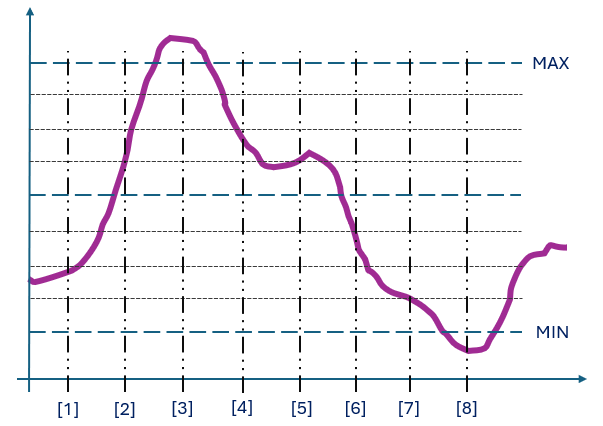
\includegraphics[width=0.7\textwidth]{images/can_signal.png}
\end{center}

On souhaite l'encoder sur sur 8 niveaux entre les valeurs \textsl{MIN} et \textsl{MAX}. Les échantillons [i] sont pris à intervalle régulier



\begin{enumerate}
	\item Combien de bits faut-il pour transmettre un échantillon ?
	\item Graduer l'axe des ordonnées avec les valeurs obtenues en sortie du convertisseur analogique-numérique (valeurs binaire et décimale).
	\item Quelles sont les valeurs binaires et décimales des 8 premiers échantillons ?
\end{enumerate}


\section*{Correction}

1/ Il faudra 3 bits, $2^3 = 8$.

\medskip

2/ 3/

\begin{center}
	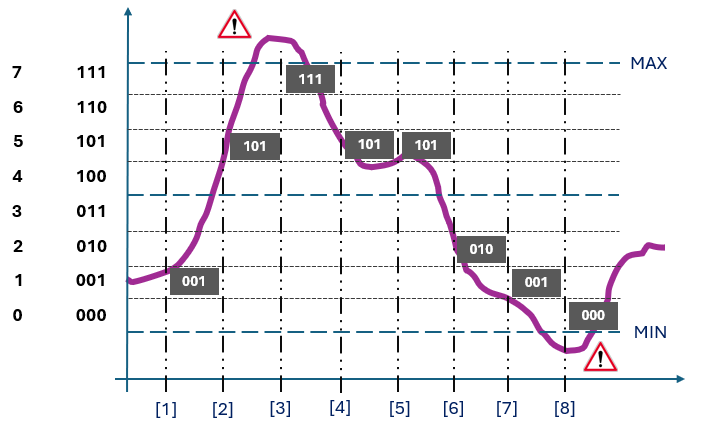
\includegraphics[width=0.7\textwidth]{images/can_signal_corr.png}
\end{center}


\newpage
%-----------------------------------
\textbf{Exercice 3 / Transmission numérique}

On souhaite transmettre des informations binaires sur une fibre. Le laser d'émission peut être piloté selon 4 niveaux d'intensité lumineuse. On ajoute également la possibilité de choisir 2 états de polarisation. 

\textit{On supposera que le délai de changement de niveaux de luminosité et de polarisation n'est pas un facteur limitant de la transmission.}

\begin{enumerate}
	\item Quelle est la \textbf{valence} de ce mode de transmission ?
	\item Quelle est la \textbf{quantité de bits transmis} par motif ?
	\item Chaque motif reste un temps $\Delta_T$ sur la fibre. En déduire le \textbf{débit binaire} en bits/s puis en octets/s. 
	
	\medskip	
	
	AN : $\Delta_T = 100\operatorname{ns}$
\end{enumerate}


\section*{Correction}

1/ La \textbf{valence} correspond au nombre de motifs différents qu'il est possible de transmettre indépendamment (nombre d'états possibles d'un signal transmis) : ici il y a 4 x 2 motifs possibles, soient 8 motifs.  \textbf{$v = 8$}

\medskip

2/ Pour pouvoir coder 8 motifs différents, \textbf{3 bits} sont nécessaires ($n = log_2(v)$).

\medskip

3/ On peut noter $R$ la rapidité de modulation (en bauds) : $R = 1 / \Delta_T$

Le débit binaire vaut : $D = n \cdot R$ 

Ici : $D = n / \Delta_T = 3 / 10^{-7} = 30 \cdot 10^6 = 30\operatorname{Mbits/s} = 3.75\operatorname{Mo/s}$


\newpage
\centerline {\rule{.70\linewidth}{.25pt}} % Horizontal line
%-----------------------------------
\textbf{Exercice 4 / Conversion numérique-analogique}

\textbf{Montage R-2R}

On s'intéresse à ce montage :

\begin{center}
	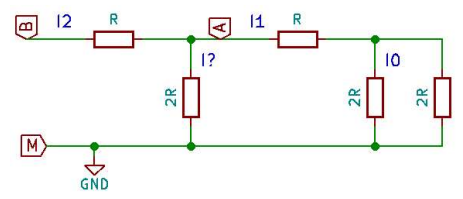
\includegraphics[width=0.5\textwidth]{images/R_2R.png}
\end{center}

\begin{enumerate}
	\item Que vaut le courant $I_1$ en fonction du courant $I_0$ (courant passant par la résistance $2R$) ?
	\item Que vaut le courant $I_2$ en fonction du courant $I_0$ (courant passant par la résistance $2R$) ?
\end{enumerate}

\section*{Correction}

1/  On peut s'intéresser à la résistance équivalente entre les points A et M.

	On trouve entre A et M une résistance $R$ en série avec un ensemble en parallèle de 2 résistances de $2R$.
	
	$R_{AM} = R + (2R // 2R)$  avec $2R//2R = \frac{2R \cdot 2R}{2R + 2R} = R$
	
	On a alors : $R_{AM} = R + R = 2R$.

\medskip

Les deux résistances de $2R$ étant en parallèle, elles sont soumises à la même différence de potentiel. Comme elles ont également la même résistance, elles sont traversées par le même courant.

La loi des noeuds au point d'intersection de $R$ et des deux résistances de $2R$ donne que $I_1 = 2 \cdot I_0$.

\bigskip

2/ En reprenant le modèle équivalent du montage entre A et M, on obtient alors un nouveau montage R-2R.

On a alors $R_{BM} = R + (2R // 2R) = 2R$. Et ainsi de suite...

De la même façon que précédemment, on obtient $I_2 = 2 \cdot I_1 = 2^2 \cdot I_0$.

En généralisant, le courant : $$I_n = 2^{n+1} \cdot I_0$$


\newpage
\textbf{Montage complet}

On s'intéresse à présent au montage suivant :

\begin{center}
	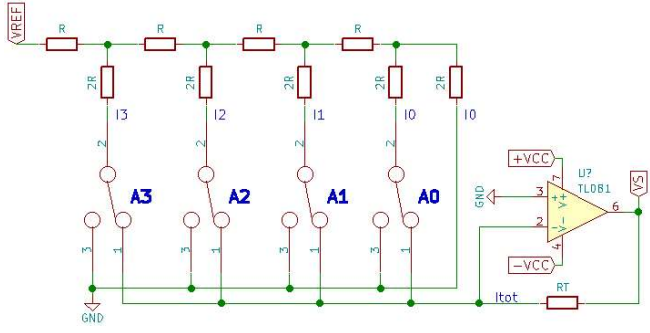
\includegraphics[width=0.8\textwidth]{images/R_2R_complet.png}
\end{center}

On supposera que lorsque $A_i = 0$, l'interrupteur $i$ est en position 3 et que lorsque Ai = 1, l'interrupteur $i$ est en position 1.

\begin{enumerate}
	\item Quel est le type de montage autour de l'ALI ?
	\item En quoi la structure vue précédemment peut nous aider ?
	\item Que vaut alors le courant $I_{tot}$ dans la contre-réaction de l'ALI en fonction des courants $I_i$ ?
	\item Que vaut alors le courant $I_{tot}$ dans la contre-réaction de l'ALI en fonction du courant $I_0$ et des
valeurs des $A_i$ ?
\end{enumerate}


\section*{Correction}

1/ Il s'agit d'un montage transimpédance, qui permet de transformer $I_{tot}$ en une tension $V_S = - R_T \cdot I_{tot}$.

\medskip

2/ On remarque que la structure est de type R-2R.

	En fonction de la position des $A_i$, le courant résultant des différentes branches va soit à la masse, soit dans le contre-réaction de l'ALI. Comme l'ALI est en mode linéaire, on a $V+ = V-$ et $V+ = 0$. Dans les deux cas, la masse est présente sur les interrupteurs $A_i$.

\medskip

3/ Si on calcule le courant au noeud en $V-$, on a $I_{tot} = A_0 \cdot I_0 + A_1 \cdot I_1 + A_2 \cdot I_2 + A_3 \cdot I_3$.
	
	De manière généralisée : 
	
	$$I_{tot} = \sum_{k = 0}^{N} A_k\cdot I_k$$
	
\medskip
	
4/ D'après la section précédente, on a vu que $I_1 = 2^1 \cdot I_0$, que $I_2 = 2^2 \cdot I_0$...
	
	On a alors : $$I_{tot} = I_0 \cdot \sum_{k = 0}^{N} A_k\cdot 2^k$$


\end{document} 